% q0066.tex — A Clean Cut at the Clinic
\question{
  id        = {0066},
  title     = {A Clean Cut at the Clinic},
  source    = {OBECON},
  year      = {2026},
  round     = {Seletiva IEO -- Phase C},
  language  = {English},
  topic     = {Micro},
  subtopic  = {Price Elasticity / Regression Discontinuity Design},
  type      = {dissertative},
  statement = {%
    A health economist studies how price affects clinic visits. Patients born
    before January~1, 1970 receive a 10\% discount on the clinic fee; those
    born after pay full price. The figure below shows average annual visits
    by birth date around the January~1, 1970 cutoff.

    \begin{center}
    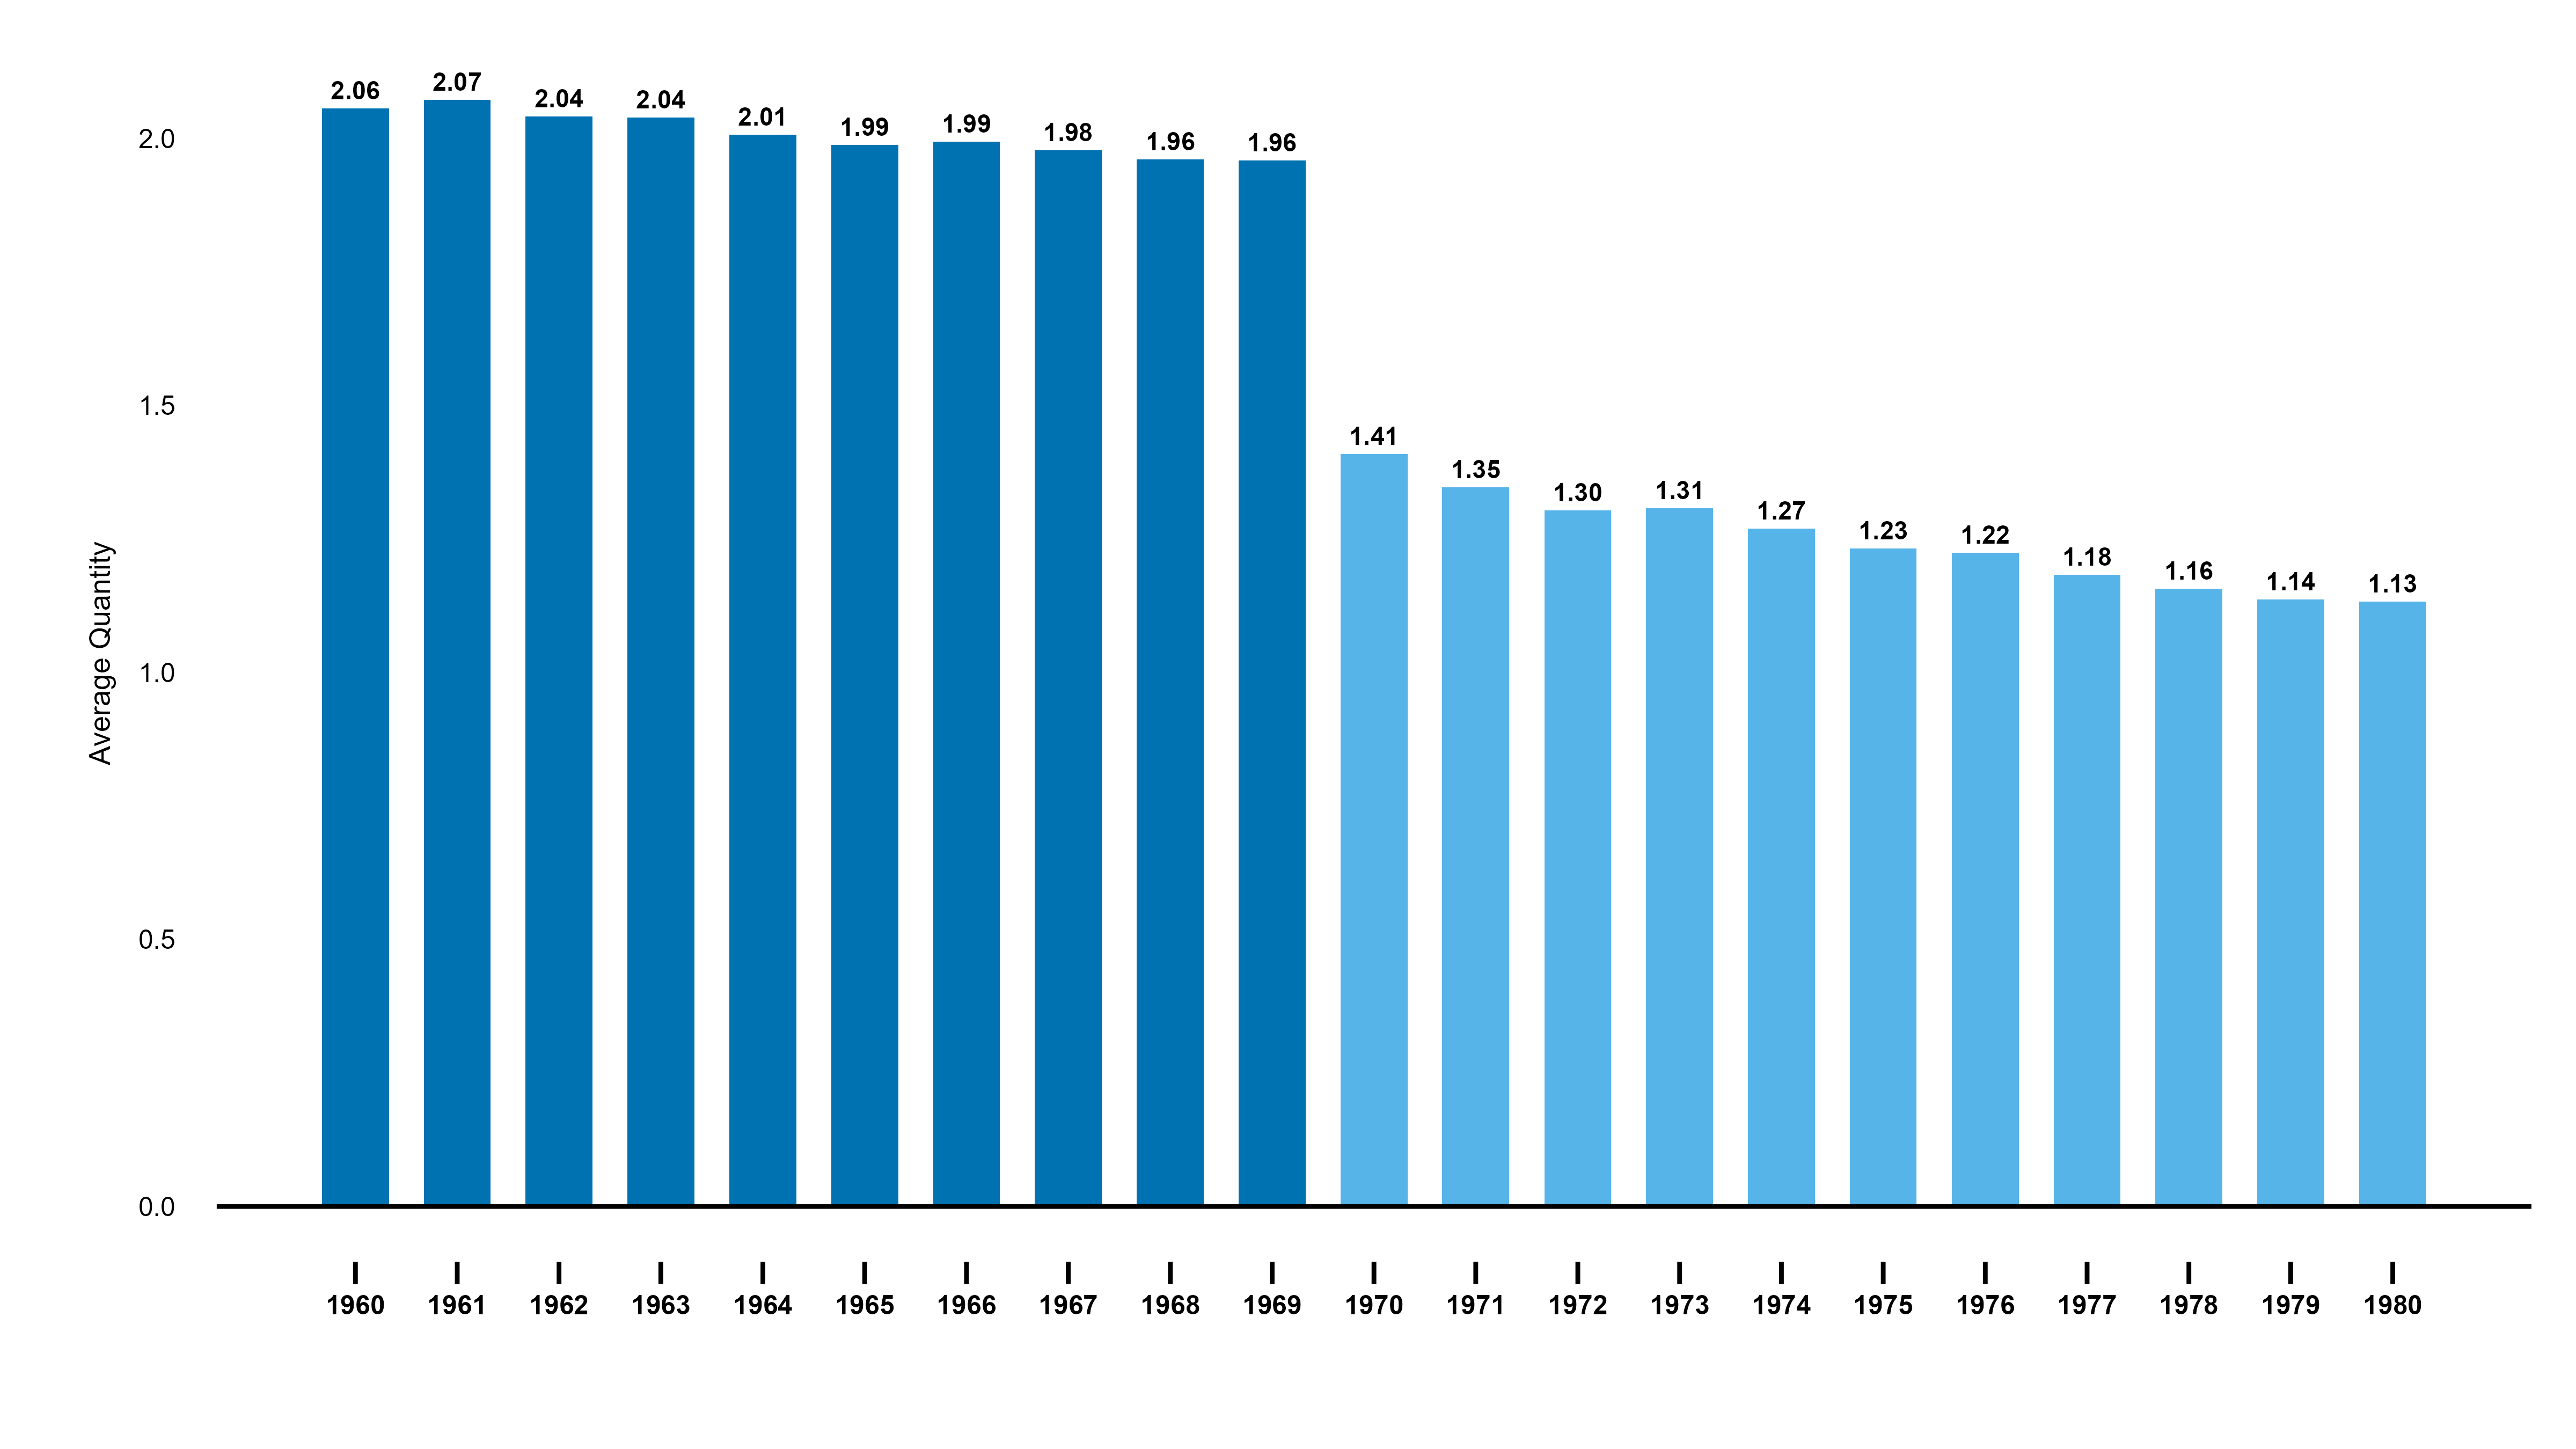
\includegraphics[width=0.80\textwidth]{../images/q0066_fig1.png}
    \end{center}

    \begin{enumerate}[(a)]
      \item (30 points) Define the price elasticity of demand. Why would a
            simple comparison of high-price vs.\ low-price patients give a
            biased estimate of the price effect?

      \item (30 points) Using the regression discontinuity design (RDD) at
            the January~1, 1970 cutoff, calculate the price elasticity of
            demand for clinic visits. Average visits just before the cutoff:
            1.96/year; just after: 1.41/year. Interpret the magnitude.

      \item (40 points) State the key assumptions required for a causal
            interpretation of the RDD estimate. Identify one plausible threat
            to validity and explain what it would mean for the estimate.
    \end{enumerate}
  },
  choices   = {},
  answer    = {},
  solution  = {%
    \textbf{(a)} Price elasticity of demand:
    \[
      \varepsilon = \frac{\%\,\Delta Q}{\%\,\Delta P}
      = \frac{\Delta Q / Q}{\Delta P / P}.
    \]
    A simple comparison is biased because patients paying different prices
    are not randomly selected (selection bias): wealthier or sicker patients
    may systematically choose different price tiers, confounding the pure
    price effect.

    \textbf{(b)} Price change at cutoff: $-10\%$ (discount for pre-cutoff
    patients). Quantity change: $(1.96-1.41)/1.41 \approx 39\%$. Elasticity:
    \[
      \varepsilon = \frac{39\%}{-10\%} \approx -3.9.
    \]
    Demand is \textbf{highly elastic}: a 1\% price decrease leads to a
    $\approx 3.9\%$ increase in visits. Patients are very sensitive to price
    changes for clinic services.

    \textbf{(c)} Key assumptions:
    \begin{itemize}
      \item \textbf{Continuity}: individuals born just before and after the
            cutoff are similar in all characteristics except discount
            eligibility.
      \item \textbf{No manipulation}: individuals cannot alter their
            birthdate to gain eligibility.
      \item \textbf{Relevance}: the discount actually creates a price
            difference at the cutoff.
    \end{itemize}
    \textit{Threat}: if another policy change coincided with the January~1,
    1970 cutoff (e.g.\ a change in insurance coverage), the estimate would
    capture both effects, invalidating the causal interpretation.
  },
}
